 
\chapter{Discusión}
\label{discus}

En el presente trabajo se lleva a cabo una propuesta preliminar de un protocolo para evaluar la eficiencia de brasinoesteroides sint\'eticos sobre la actividad de tres enzimas de defensa en plantas.  \\ 

La selecci\'on de \textit{Raphanus sativus} como modelo experimental se bas\'o en los numerosos trabajos cient\'ificos que detectan el incremento de la actividad de las enzimas de defensa, ante aplicaciones ex\'ogenas de BRs, aumentando as\'i la tolerancia de las plantas frente a distintos tipos de estr\'es. Por ejemplo, \cite{mahesh2013effect} utilizaron \textit{R. sativus} como modelo para analizar el efecto de dos an\'alogos de BRs (24-EpiBL y 28-HomoBL) y observaron el aumento de la actividad de enzimas antioxidantes, lo que disminuy\'o el efecto inhibitorio causado por estr\'es h\'idrico. \cite{anuradha2007effect} indican c\'omo al tratar plantas sometidas a estr\'es por Cadmio (Cd) con 24-EpiBL y 28-HomoBL aumenta la actividad de las enzimas antioxidantes SOD y CAT. La 24-EpiBL disminuy\'o los efectos de toxicidad del Cadmio (Cd) y el Mercurio (Hg), mediante la modulaci\'on de la actividad de enzimas antioxidantes, como SOD y CAT \citep{dhriti201424}; adem\'as, disminuy\'o el estr\'es oxidativo a trav\'es del incremento de la actividad de las enzimas de defensa, incluyendo PPO \citep{sharma2012effect}. \cite{ramakrishna2013preliminary} identificaron el aumento de la tolerancia en plantas de \textit{R. sativus} ante toxicidad por Zinc (Zn) al incrementar la actividad de enzimas antioxidantes, como resultado de la aplicaci\'on de 28-homoBL. Adem\'as, \cite{choudhary2012chromium} comprobaron que plantas de \textit{R. sativus} sometidas a estr\'es por Cobre (Cu), al ser tratadas con BRs ex\'ogenos pose\'ian mayor acumulaci\'on de enzimas antioxidantes.\\

En este trabajo se proponen dos dise\~nos experimentales que permiten la posterior evaluaci\'on de la actividad de las enzimas de defensa en plantas de \textit{R. sativus} y el efecto que pueden ejercer los an\'alogos sint\'eticos de BRs sobre la  actividad de las mismas. El protocolo propuesto permitir\'a determinar si existen diferencias en las respuestas generadas al aplicar los compuestos DI-31 y MH-5 en plantas sometidas a estr\'es salino, o no sometidas a este. \\

Existen diferentes v\'ias de aplicaci\'on ex\'ogena de BRs, entre las que se incluyen incubaci\'on de la semilla en el compuesto, tratamientos en las ra\'ices y aspersión foliar \citep{yusuf2019interplay}. Con el objetivo de evaluar si este elemento tiene influencia en el efecto de los tratamientos, se proponen dos v\'ias diferentes (aspersi\'on foliar e incubaci\'on de la semilla en el compuesto), lo que permitir\'a establecer cu\'al de estas es m\'as efectiva para desencadenar la respuesta de defensa. \\ 

%Entre los dise\~nos experimentales, el por qu\'e se decidi\'o probar un segundo m\'etodo en el que se sometieran las plantas a estr\'es previamente (ver el art\'iculo espec\'ifico por el cual vimos esto), al tener la consideraci\'on que probablemente las enzimas aumentar\'ian m\'as ante la inducci\'on de estr\'es por salinidad a pesar de que las ROS se encuentran tanto en plantas con estr\'es como en las que se encuentran en su estado basal. De todas formas el estr\'es por salinidad es una forma de retar la planta. \\


\section{Determinaci\'on de la cantidad de prote\'inas.}

El m\'etodo de cuantificaci\'on de prote\'inas Bradford descrito por primera vez por \cite{bradford1976rapid}, es una metodolog\'ia r\'apida, simple y certera para estimar la concentraci\'on de prote\'inas \citep{kruger2009bradford}. El colorante CBBG existe en dos formas de coloraci\'on diferente, rojo y azul. La forma roja es convertida a la azul al unirse el CBBG a la prote\'ina, lo que produce un incremento de absorci\'on de $465$ a $595\;nm$, que es monitoreado espectrofotom\'etricamente \citep{bradford1976rapid}. \\

El colorante se une más fácilmente a los residuos de arginina y lisina de las proteínas \citep{compton1985mechanism, congdon1993binding}. Esta especificidad puede conducir a variaciones en los resultados del ensayo frente a proteínas diferentes, siendo este el principal inconveniente del m\'etodo. El m\'etodo original de Bradford muestra gran variaci\'on en la respuesta a diferentes prote\'inas \citep{read1981minimization, friedenauer1989sensitivity, stoscheck1990increased}. Para solucionar este problema se han realizado numerosas variaciones a la metodolog\'ia, sin embargo, estos cambios generalmente resultan en un ensayo menos robusto, que a menudo es m\'as susceptible a interferencias. Consecuentemente, el método original ideado por \cite{bradford1976rapid} sigue siendo el m\'as conveniente y ampliamente  utilizado \citep{kruger2009bradford}. \\

Aunque los resultados del an\'alisis de varianza con los datos de concentración de proteínas fueron no significativos entre los distintos tiempos del experimento, a medida que pasa el tiempo disminuye la concentración de proteínas, por lo que los ensayos no se deben prolongar hasta cuatro d\'ias. \\

\section{Enzima Super\'oxido Dismutasa (SOD).}

%Comparaci\'on entre los resultados arrojados por cada uno de los protocolos de SOD, en este caso, se discute el mecanismo de la medici\'on mediante el reactivo pyrogallol y como la presencia de pigmentos puede haber influido en los resultados err\'oneos y como finalmente al extraer con acetona (explicar brevemente el m\'etodo con acetona como funciona) resuelve el problema de los pigmentos y los resultados en las curvas dan en el sentido correcto. \\

El m\'etodo de determinaci\'on de la actividad enzim\'atica de SOD, mediante la inhibici\'on de la autoxidaci\'on del Pyrogallol es uno de los m\'as utilizados, sin embargo, en la literatura se observan diferencias en las condiciones de ensayo empleadas. Por ejemplo, hay variaciones en la longitud de onda, la adici\'on o no de EDTA, el pH de la soluci\'on tamp\'on Tris-HCl, el solvente, el tiempo de ensayo y la temperatura, por lo que existen tambi\'en variaciones en los resultados obtenidos \citep{zhang2016optimization}. \\

El Pyrogallol se autoxida r\'apidamente en soluciones alcalinas, formando gran n\'umero de productos intermedios, cuya aparici\'on puede ser medida a $420\;nm$ (Fig. \ref{pyr}) \citep{marklund1974involvement}. La habilidad de SOD de inhibir la autoxidaci\'on del Pyrogallol (al generar super\'oxido) ha sido empleada de forma exitosa para la cuantificaci\'on de esta enzima. El Pyrogallol es un buen reductor de hierro (Fe) y el hierro reducido se puede autoxidar r\'apidamente generando radicales hidroxilo, lo que produce interferencias en el ensayo. La adici\'on de agentes quelantes como DETAPAC y EDTA en la mezcla del ensayo, elimina la posibilidad de interferencias de los iones $Fe^{2+}$, $Cu^{2+}$ y $Mn^{2+}$ \citep{pandey2014oxidative}, aunque pueden existir interferencias peque\~nas de $Fe^{2+}$ \citep{misra1972role, marklund1974involvement}. \\

\begin{figure}[hbtp]
	\centering
	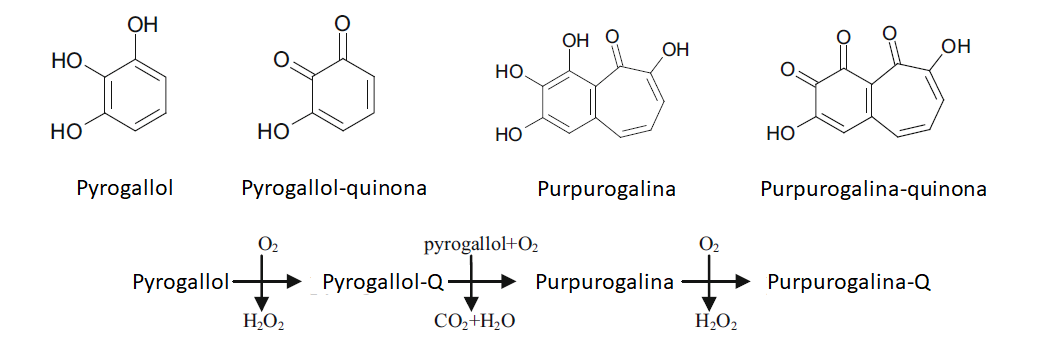
\includegraphics[scale=0.6]{Imagenes/pyr}
	\caption{Productos y secuencia de reacci\'on del Pyrogallol. Modificado de \cite{ramasarma2015new}.}
	\label{pyr}
\end{figure}

La velocidad de autoxidaci\'on del Pyrogallol depende fuertemente de su concentraci\'on y del pH. Adem\'as, existen otras mol\'eculas redox de bajo peso molecular que pueden reaccionar directamente con el diox\'igeno, aumentando la velocidad de autoxidaci\'on del Pyrogallol \citep{gao1998mechanism}. \\



%Cuando el radical superóxido se acumula y produce la autooxidación del pirogalol da lugar a la formación de purpurogalina, un compuesto amarillo-marrón con un pico máximo de absorbancia de luz a 420 nm y coeficiente de extinción molar 2640 M?¹cm?¹. Cuando hay SOD presente en el medio, la enzima compite con el pirogalol por el radical superóxido, inhibiéndose la reacción de autooxidación, lo que implica menor formación de purpurogalina. La formación de purpurogalina es susceptible de ser medida espectrofotométricamente en el tiempo, con lo que se puede aprovechar el fenómeno para cuantificar la actividad SOD de una muestra problema midiendo la inhibición de la autooxidación del pirogalol respecto de un control

En las tablas \ref{24hSOD}, \ref{48hSOD} y \ref{96hSOD} se observa que la velocidad de autoxidaci\'on del Pyrogallol en la soluci\'on tamp\'on,  siempre es menor o igual que la velocidad para los extractos, por lo que aparentemente no se produce inhibici\'on de la autoxidaci\'on del Pyrogallol, que te\'oricamente deber\'ia existir producto de la actividad de SOD. Esto se puede deber a interferencias de algunos de los componentes del extracto que determinan una mayor autoxidación de la que la enzima puede contrarrestar. \\

La adición de EDTA en mayor proporción no cambi\'o el  resultado obtenido, luego la presencia de algún catión divalente no autoxidaba el sustrato. Por tanto, 1mM de EDTA es suficiente para impedir la influencia de estos cationes, lo que se corresponde con lo indicado por \cite{marklund1974involvement}. \\

El protocolo de extracción con acetona \citep{baquero2005catalase} eliminaría las interferencias de pigmentos, por lo que se decidi\'o extraer la enzima mediante este protocolo y evaluar la actividad de SOD en este extracto.\\

La técnica de extracción enzim\'atica con acetona  empleada en este trabajo se basó en reportes previos, en los que se obtenía una buena eficiencia en la extracción de proteína y en la actividad enzimática \citep{sala1999catalase,  narvaez2002evaluacion, camelo2004polifenoloxidasa}. Los polvos de acetona permiten que el extracto presente una alta actividad con una mayor estabilidad, además de evitar la inactivación enzimática durante la extracción, porque con la acetona se retiran los fenoles, $\beta$-carotenos y ácidos orgánicos del extracto, disminuyendo así la reacción de las enzimas con estos compuestos \citep{baquero2005catalase}. Otros art\'iculos, por ejemplo \cite{lopez2014actividad} tambi\'en emplean protocolos de extracci\'on similares. \\

Dado los resultados obtenidos en el presente trabajo, es probable que la causa del incremento de la autoxidaci\'on del Pyrogallol sea la presencia de sustancias como fenoles, $\beta$-carotenos y ácidos orgánicos. Los extractos obtenidos mediante el protocolo de extracci\'on de \cite{baquero2005catalase} (con modificaciones) presentaron actividad de la enzima SOD, aunque por este protocolo hay una p\'erdida importante de prote\'inas.\\


\section{Enzima Catalasa (CAT)}

%En el caso de CAT TODAS las consideraciones que hay que tener encuenta para medir esta enzima. En los art\'iculos que est\'an en la literatura solo miden 2 puntos y asumen que la enzima tiene un comportamiento lineal, pero realmente en niguno de los art\'iculos miden m\'as de dos puntos, solo en el tiempo inicial y en el final y se restan ambos puntos. No observan la linealidad de la enzima. 

La metodolog\'ia m\'as utilizada para medir la actividad de la enzima CAT es la medici\'on espectrofotom\'etrica del cambio de absorbancia a $240\;nm$ ante altos niveles de per\'oxido de hidr\'ogeno (mayores o iguales a $30\;mM$). Los altos niveles de per\'oxido de hidr\'ogeno llevan inmediatamente a la inhibici\'on de la enzima CAT, alterando la estructura de su centro activo. Existe la necesidad de un m\'etodo para evaluar continuamente la baja actividad de la enzima CAT frente a un fondo de alto nivel de absorbancia que se produce debido a que muchos constituyentes celulares, como \'acidos nucleicos y prote\'inas exhiben una intensa absorci\'on a $240\;nm$ \citep{hadwan2018simple}.\\

La cin\'etica de la CAT no sigue un patr\'on usual. Primeramente, no es posible saturar la enzima con sustrato dentro del intervalo de concentraciones menores a $5\;M$ de per\'oxido de hidr\'ogeno. Por otra parte, a concentraciones mayores de $0.1\;M$ ocurre una r\'apida inactivaci\'on de la enzima. En consecuencia, la determinaci\'on de la actividad a concentraciones saturantes, no es posibles. En contraste a las reacciones que se desarrollan a concentraciones saturantes de sustrato, la descomposici\'on enzim\'atica del per\'oxido de hidr\'ogeno es una reacci\'on de primer orden, por lo que la tasa de reacci\'on es proporcional a la cantidad de per\'oxido de hidr\'ogeno presente. Para evitar una r\'apida disminuci\'on en la tasa inicial de la reacci\'on, esta se debe llevar a cabo con concentraciones de $H_2O_2$ bajas (alrededor de $0.01\;M$) \citep{aebi198413}.\\

Este trabajo condujo a la identificaci\'on de posibles causas de errores en la medici\'on de la CAT. Por ejemplo, el extracto enzim\'atico debe ser adicionado y al instante realizar la medici\'on espectrofotom\'etrica, que debe realizarse espec\'ificamente en cubetas de cuarzo. El pH debe ser controlado y es necesario evitar que el extracto enzim\'atico experimente procesos de congelaci\'on-descongelaci\'on. Adem\'as se debe comprobar que no existan burbujas en las paredes de la cubeta. \\ 

%Art\'iculos a citar donde solo miden 2 puntos a 15 y 180 segundos:
%
%\citep{lopez2014actividad}

\section{Enzima Polifenol Oxidasa (PPO).}

%- En el caso de PPO ver el logro de realizar este protocolo en placas, pues el extracto es limitado. Ver que con el extracto de acetona no funciona. Ver lo del art\'iculo del dise\~no 2 que explica los resultados que tenemos.\\ 

El compuesto L-DOPA posee un gran potencial como sustrato modelo para estudios de la degradaci\'on enzim\'atica de compuestos fen\'olicos. En presencia de la enzima PPO es convertido r\'apidamente a 2-carboxi 2,3-dihidroindol 5,6-quinona, que puede ser medido espectrofotom\'etricamente a $475\;nm$ \citep{pind1994enzymic}.\\

La PPO es una de las enzimas responsables de la oxidaci\'on de compuestos fen\'olicos \citep{sheen1969studies} y la disminuci\'on de su actividad puede inducir una acumulaci\'on de fenoles totales \citep{das1992sodium}. \cite{muthukumarasamy2000enhancement} comprobaron que la actividad enzim\'atica de PPO en plantas, disminuye ante e estr\'es por salinidad, lo que puede llevar al da\~no oxidativo. \\

Al comparar los valores de $K_ma$ de las plantas que germinaron a partir de semillas que no fueron incubadas en agua previo a su siembra (Fig. \ref{POd1}) con los valores de semillas que si fueron incubadas en agua (Fig. \ref{a}), podemos observar como la incubaci\'on afecta positivamente el valor de este par\'ametro, lo que coincide con los informes encontrados en la literatura \citep{burgass1984evidence, bradford1986manipulation, taylor1998seed, mcdonald2000seed}. En el caso de $V_{max}$ las plantas de semillas que no fueron incubadas en agua previo a su siembra (Fig. \ref{POd1}), mostraron un valor mayor de este par\'ametro que las plantas incubadas en agua y las sometidas a estr\'es salino (Fig. \ref{POkmVmax}). No se puede llegar a conclusiones reales a partir de los valores obtenidos, pues se trata de ensayos puntuales, en los que no se pueden realizar an\'alisis estad\'isticos.\\


En el trabajo realizado la variaci\'on entre los valores de $V_{max}$ de plantas sometidas a estr\'es por salinidad y su control negativo fue peque\~na, como se puede observar en la figura \ref{1}.\\

Por su parte los valores obtenidos de $K_ma$ mostraron una mayor variaci\'on. En este caso, como se muestra en la figura \ref{2}, los extractos obtenidos a partir de plantas de \textit{R. sativus} sometidas a estr\'es presentaron un valor de $K_ma$ mayor, con respecto al control negativo, lo que pudiese indicar aumentos de la afinidad de la enzima por el sustrato en respuesta al estr\'es salino.\\

Al medir la actividad enzim\'atica de PPO en extractos realizados seg\'un la metodolog\'ia de extracci\'on de \cite{baquero2005catalase}, no se observ\'o actividad de la enzima. En este sentido, se recomienda utilizar otra soluci\'on tamp\'on para diluir el precipitado proteico formado en el ensayo y la utilizaci\'on de un sustrato diferente, por ejemplo: catecol \citep{martinez2013actividad}.



